\newpage
\section{Maciej Cieżak}
\label{mciezak}

Here is a picture of a mantis shrimp (Figure \ref{fig:ms})

\begin{figure}[h]
    \centering
    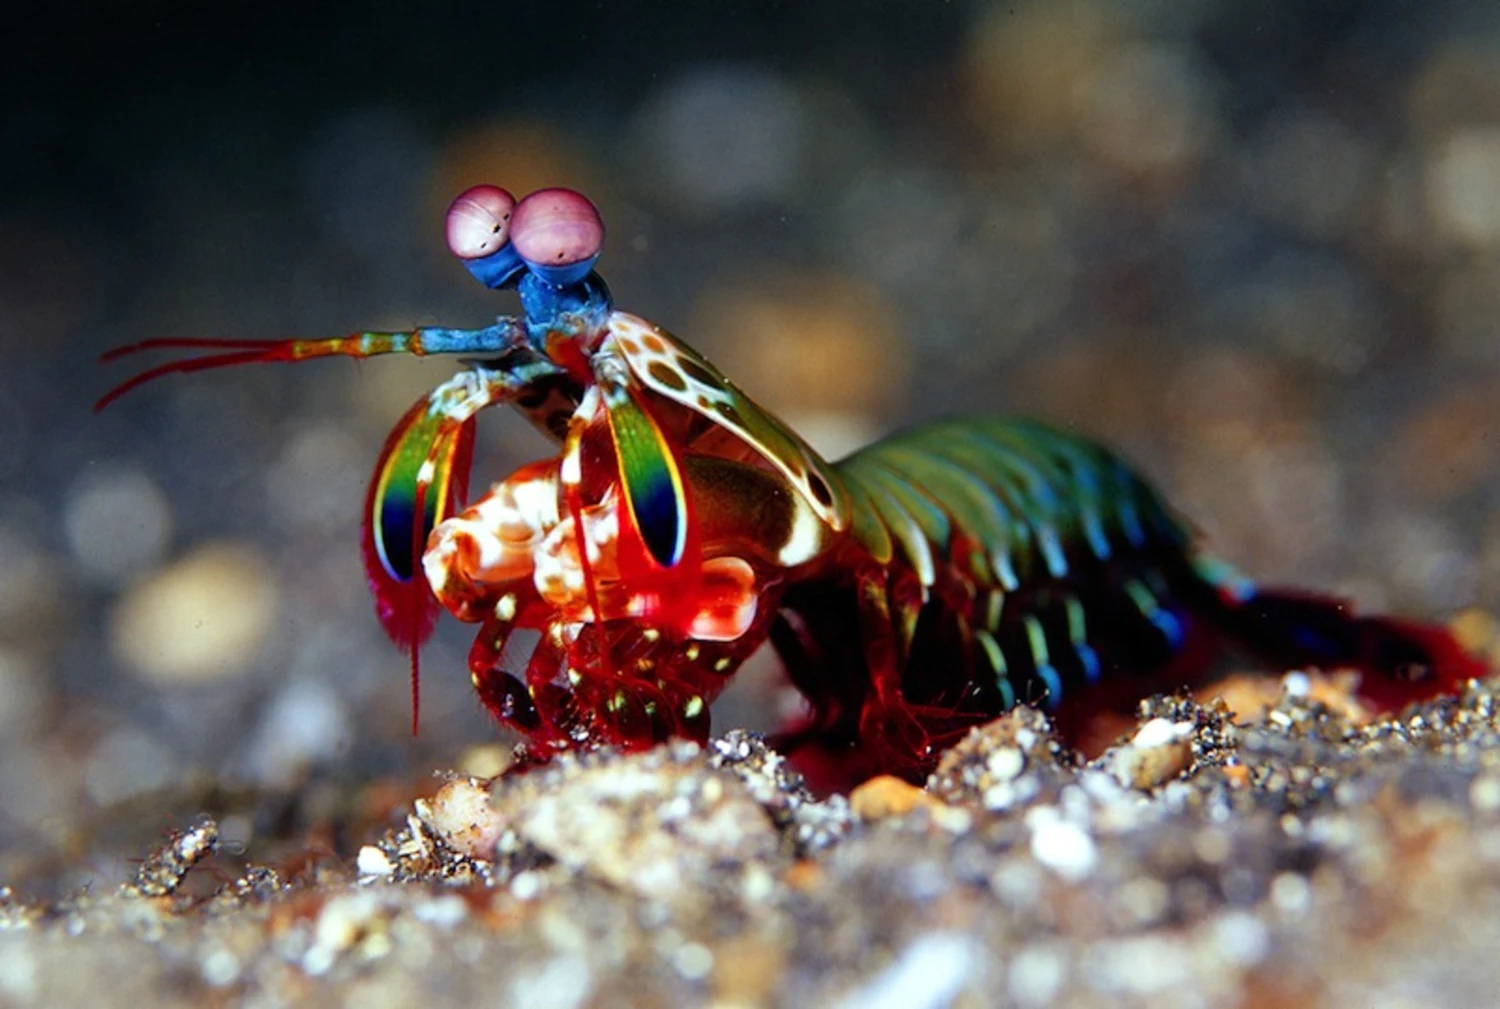
\includegraphics[width=12cm]{Pictures/ms.png}
    \caption{A mantis shrimp}
    \label{fig:ms}
\end{figure}

\hrulefill

\begin{align}
    \textbf{Mantis shrimp} are carnivorous marine crustaceans of the order \textbf{Stomatopoda}. Stomatopods branched off from other members of the class Malacostraca around \underline{340 million years} ago. Mantis shrimp typically grow to around 10 cm (3.9 in) in length, while a few can reach up to 38 cm (15 in). A mantis shrimp's carapace covers only the rear part of the head and the first four segments of the thorax. Varieties range in colour from shades of brown to vivid colours, with more than \underline{520 species} of mantis shrimp known. They are among the most important predators in many shallow, tropical and subtropical marine habitats. However, despite being common, they are poorly understood, as many species spend most of their lives sheltering in burrows and holes.
    \par Called "sea locusts" by ancient Assyrians, "prawn killers" in Australia, and now sometimes referred to as "thumb splitters"—because of the animal's ability to inflict painful wounds if handled incautiously—mantis shrimp have powerful raptorial appendages that are used to attack and kill prey either by spearing, stunning, or dismembering. Some mantis shrimp species have specialised calcified 'clubs' that can strike with great power, while others have sharp forelimbs used to seize the prey (hence the term "mantis" in their common name).
\end{align}

\newpage

\textbf{Scientific classification:}
\begin{flushleft}
\begin{tabular}{ || c | c || } 
 \hline
 Domain & Eukaryota \\ 
 \hline
 Kingdom & Animalia \\ 
 \hline
 Phylum & Arthropoda \\ 
 \hline
 Class & Malacostraca \\
 \hline
 Subclass & Hoplocarida \\
 \hline
 Order & Stomatopoda \\
 \hline
\end{tabular}
\end{flushleft}

\textbf{Example species:}
\begin{itemize}

   \item Family Gonodactylidae
   \begin{itemize}
     \item Gonodactylus smithii
   \end{itemize}
   
   \item Family Hemisquillidae
   \begin{itemize}
     \item Hemisquilla ensigera
     \item Hemisquilla australiensis
     \item Hemisquilla braziliensis
     \item Hemisquilla californiensis
   \end{itemize}
   
   \item Family Lysiosquillidae
   \begin{itemize}
     \item Lysiosquillina maculata
   \end{itemize}

   \item Family Nannosquillidae
   \begin{itemize}
     \item Nannosquilla decemspinosa
     \item Platysquilla eusebia
   \end{itemize}

   \item Family Odontodactylidae
   \begin{itemize}
     \item Odontodactylus scyllarus
     \item Odontodactylus latirostris
   \end{itemize}

   \item Family Pseudosquillidae
   \begin{itemize}
     \item Pseudosquilla ciliata
   \end{itemize}

   \item Family Squillidae
   \begin{itemize}
     \item Oratosquilla oratoria
     \item Rissoides desmaresti
     \item Squilla empusa
     \item Squilla mantis
   \end{itemize}

   \item Family Tetrasquillidae
   \begin{itemize}
     \item Heterosquilla tricarinata
   \end{itemize}
   
\end{itemize}

\newpage
\begin{align}
    The mantis shrimp's second pair of thoracic appendages has been highly adapted for powerful close-range combat. The appendage differences divide mantis shrimp into two main types: those that hunt by impaling their prey with spear-like structures and those that smash prey with a powerful blow from a heavily mineralised club-like appendage. A considerable amount of damage can be inflicted after impact with these robust, hammer-like claws. This club is further divided into three subregions: the impact region, the periodic region, and the striated region. Mantis shrimp are commonly separated into many (most fall into spears and smashers but there are some outliers) distinct groups determined by the type of claws they possess:
\end{align}
\begin{description}
     \item [Smashers] - possess a much more developed club and a more rudimentary spear (which is nevertheless quite sharp and still used in fights between their own kind); the club is used to bludgeon and smash their meals apart. The inner aspect of the terminal portion of the appendage can also possess a sharp edge, used to cut prey while the mantis shrimp swims.
     \item [Spearers] - are armed with spiny appendages - the spines having barbed tips - used to stab and snag prey.
\end{description}
\begin{align}
    Both types strike by rapidly unfolding and swinging their raptorial claws at the prey, and can inflict serious damage on victims significantly greater in size than themselves. In smashers, these two weapons are employed with blinding quickness, with an acceleration of \underline{10,400 g (102,000 m/s²)} and speeds of \underline{23 m/s (83 km/h)} from a standing start. Because they strike so rapidly, they generate vapor-filled bubbles in the water between the appendage and the striking surface—known as cavitation bubbles. The collapse of these cavitation bubbles produces measurable forces on their prey in addition to the instantaneous forces of \underline{1,500 newtons} that are caused by the impact of the appendage against the striking surface, which means that the prey is hit twice by a single strike; first by the claw and then by the collapsing cavitation bubbles that immediately follow. Even if the initial strike misses the prey, the resulting shock wave can be enough to stun or kill. \\
    To better understand underlined numbers here is a reminder of the formulas:
\end{align}
\[V = \frac{s}{t}\]
\[a = \frac{\Delta{V}}{\Delta{t}}\]
\[F = am\]